\documentclass[12pt,a4paper]{report}
\date{}
\usepackage[hmargin={1.15in,1in},vmargin={1in,1.1in},]{geometry}
%\usepackage[hmargin={1.5in,1.25in},vmargin={1in,1in},]{geometry}
\usepackage{amsmath,graphicx,makeidx,listings,subfigure,float,setspace}
\usepackage{fancyhdr}
\thispagestyle{empty}
\usepackage{sectsty}
\usepackage{lipsum}
%\usepackage[center]{titlesec}
\usepackage[final]{pdfpages}
\usepackage{titlesec}
\renewcommand\listfigurename{\Huge \begin{center} {List of Figures} \end{center} }
\renewcommand{\contentsname}{ \begin{center} TABLE OF CONTENTS  \end{center}}
\renewcommand\listtablename{\Large \begin {center}{LIST OF TABLES} \end{center}}

%\renewcommand\thebibliography{THEBIBLIOGRAPHY}
%---------------------------------FRONT PAGE--------------------------------------------------------------


\title{{\bf \Large AUTOMATIC FARMING ROBOT FOR SMART AND EFFECTIVE CULTIVATION  }\\    
\vspace{0.2cm}
{\normalsize {A PROJECT REPORT}}\\
\vspace{0.2cm}
{\normalsize{ submitted by}}\\
\vspace{0.20 cm}
{\normalsize\textbf{AJO ELDHO BABY}} \\
\normalsize {Reg. No :\textbf{ MAC15EC010}}\\
\vspace{0.20 cm}
{\normalsize\textbf{APHSANA SALIM}} \\
\normalsize {Reg. No :\textbf{ MAC15EC029}}\\
\vspace{0.20 cm}
{\normalsize\textbf{RIYA KURUVILLA}} \\
\normalsize {Reg. No :\textbf{ MAC15EC104}}\\
\vspace{0.20 cm}
\normalsize {\textbf{ ROSE MARY BENNY}}\\
\normalsize {Reg. No :\textbf{ MAC15EC107}}\\
\vspace{0.20 cm}
\normalsize{to}\\ 
\vspace{0.4cm}
\normalsize {the APJ Abdul Kalam Technological University}\\
\normalsize {in partial fulfillment of the requirements for the award of the Degree}\\
\vspace{0.4cm}
\normalsize {of}\\
\vspace{0.4cm}  
\normalsize {Bachelor of Technology}\\  
\normalsize {in} \\
\normalsize {\emph{  Electronics and Communication Engineering} }\\
\begin{figure}[H]
\centering
\includegraphics[scale=0.85]{ma}
\end{figure}
{\large \textbf {Department of  Electronics and Communication Engineering}}\\
\vspace{0.4cm}
\normalsize {Mar Athanasius College of Engineering}\\
\normalsize {Kothamangalam, Kerala, India 686 666}\\
\vspace{0.4cm}
\author \large {MAY 2019}}


%----------------------------------TABLE OF CONTENTS DEPTH-----------------------------------------------
%\setcounter{tocdepth}{1}
\renewcommand{\bibname}{ REFERENCES}
%-------declaration----------------------------------------

%CERTIFICATE
\begin{document}
%\begin{doublespace}
\newpage
\maketitle
\begin{center}
{\large \bf{DEPARTMENT OF ELECTRONICS AND COMMUNICATION ENGINEERING}}\\
{\large \bf{MAR ATHANASIUS COLLEGE OF ENGINEERING}}\\
{\large \bf{KOTHAMANGALAM}}
\end{center}
%\end{doublespace}
\begin{center}
\thispagestyle{empty}
\includegraphics[scale=0.9]{ma}\\[7pt]
\large{\bf{CERTIFICATE}}
\end{center}
\onehalfspacing This is to certify that the report entitled {\large{ \textbf{Automatic Farming Robot For Smart And Effective Cultivation  }}} submitted by \textbf{Mr.Ajo Eldho Baby, Ms. Aphsana Salim, Ms. Riya Kuruvilla and Ms. Rose Mary Benny} to the APJ Abdul Kalam Technological University in partial fulfillment of the requirements for the award of the Degree of Bachelor of Technology in  Electronics \&\ Communication Engineering is a bonafide record of the project work carried out by them under our guidance and supervision. This report in any form has not been submitted to any other University or Institute for any purpose.
\vspace{0.8in}
\begin{flushleft}
%.................................. \hfill {\bf ............................... }\\ 
{\large{\textbf{Dr. Jinsa Kuruvilla}}}\hfill{\large {\textbf{Dr.Mathew K}}}
\end{flushleft}

\begin{flushleft}
 %                                  \hfill {\bf ................................. }
Project guide                               \hfill{Head of the Department}
\end{flushleft}
 
%--------------------------------------ACKNOWLEDGMENT------------------------------------------------
\newpage
\pagenumbering{roman}
\setcounter{page}{1}
\begin{verbatim}
\end{verbatim}
\begin{center}
\textbf {\large ACKNOWLEDGEMENT}
\end{center}
\vspace{0.4125in}
\par
It is a great pleasure to acknowledge all those who have assisted and supported us for successfully completing our project.
\\
\par 
First of all, we thank God Almighty for his blessings as it is only through his grace that we were able to complete our project successfully.
\\
\par 
We are deeply indebted to Dr. Solly George, Principal, Mar Athanasius College of Engineering for her encouragement and support.
\\
\par
We express our deep sense of gratitude to Dr Mathew K, Head of Electronics \&\  Communication Engineering Department.
\\
\par
We also extend our deep sense of gratitude to our Project Guide, our Project Coordinator and Faculty Advisor, Dr. Jinsa Kuruvilla, Assistant Professor, Electronics \&\  Communication Engineering Department for her constant support and immense contribution for the success of our project.
\\
\par
 We whole - heartedly thank all our classmates, for their valuable suggestions and for the spirit of healthy competition that exists between us. 
 
 %-----------------------------------------ABSTRACT---------------------------------------------
 
\newpage
\begin{verbatim}
\end{verbatim}
\begin{center}
{\bf{ABSTRACT}}
\addcontentsline{toc}{chapter}{Abstract}
\end{center}
\vspace{30pt}
\begin{doublespace}
\hspace*{1cm}  The goal of this project is design and fabricate a multicopter  to obtain a stable flight with live video recording,  autonomous navigation and video analysis/processing. Technological advances have reduced the cost
and increase the performance of the low power microcontrollers which helps in developing multicopters.  This project uses a completely 3D printed frame using Poly Lactic Acid(PLA), brushless dc motors, electronic speed controllers, flight controller, transmitter and receiver, GPS module and Raspberry pi for video processing. This drone also houses a  wide angle micro first person view camera(FPV) which allows the user to control and navigate the drone beyond line of sight. For obtaining a more stable flight, hexacopter design is chosen instead of quadcopter design. It also makes use of technologies like OpenCV
(Open Computer Vision) and Python programming to implement autonomous navigation, face recognition, object detection and tracking and  obstacle avoidance. By analyzing the video captured and then comparing it with trained datasets, it is possible to identify objects/people in real time.  This enables the drone to detect criminals or missing people/item. The drone is also designed to lift high payloads upto 4-5 kgs which allows it to carry mail, parcels, medicines and fire extinguishers. By incorporating autonomous navigation, the drone will be able to reach it's destination without human aid. Object avoidance is carried out with the help of image processing using openCV along with IR sensor for better performance.  This makes this project highly useful for relief and rescue operations during natural calamities. 

\end{doublespace}


%-----------------------------TABLE OF CONTENTS-----------------------------------------------------------
\newpage
{
%\includepdf[pages={1}]{contents}
}
\tableofcontents
%\listoftables
\addtocontents{lot}{ \hspace{0.4cm} Table No. \hspace{1in} Title \hfill{Page No.}\par}
\listoffigures
\addcontentsline{toc}{chapter}{List of Figures}
\addtocontents{lof}{ \hspace{0.4cm} Figure No. \hspace{1in} Title \hfill{Page No.}\par}

%----------------------HEADER AND  FOOTER-----------------------------------------------------------------
\newpage
\pagenumbering{arabic}
\setcounter{page}{1}
\pagestyle{fancy}
\lhead{\emph{Automatic farming robot for smart and effective cultivation }}
\chead{}
\rhead{}
\lfoot{\emph{B.Tech, ECE, MACE, Kothamangalam}}
\cfoot{}
\rfoot{\thepage}
\renewcommand{\headrulewidth}{1pt}
\renewcommand{\footrulewidth}{1pt}
\renewcommand{\chaptername}{ {CHAPTER}}
%\renewcommand{\cftchapfont}{16pt}
\chapterfont{\centering}
\renewcommand\bibname{REFERENCES}
%------------INTRODUCTION---------------------------------------------------------------------------------
\titleformat{\chapter}[display]{ \filcenter \Large \bfseries}{\chaptertitlename\ \thechapter}{5pt}{\Large}
\titleformat*{\section}{\large\bfseries}

\chapter{ INTRODUCTION}

\hspace*{1cm}
Agricultural automation using FarmBot is an attempt to reduce the burden of maintaining a farm for small scale and large scale alike by automating the most commonly performed tasks such as sowing of seeds, watering of plants and finally even removing weeds .It is a precision agriculture CNC farming project consisting of a Cartesian coordinate robot farming machine. It requires electricity, internet connection and water supply which will be provided using off grid solutions including a water barrel to collect rain and battery to provide electricity.
\\\\\hspace*{1cm} 
 FarmBot move around in the XYZ space day and night, 7 days a week growing food. FarmBot precisely sows seed in any pattern and density and then water them efficiently the exact amount that each plant needs based on its type ,its age ,soil, conditions, the local weather and growing preference. FarmBot can grow a wide variety of crops all in the same area at the same time while each plant is cared for individually in an optimized automated way. By using soil senor, the water content of the soil and other necessary information are taken. By analyzing the data, the water sprinkler through which water, fertilizer and pesticide solutions can be sprayed, sprays the liquid by coming to the right coordinate. The camera which is fixed on the moving arm will continuously monitor for plants other than the planted ones, and also provide an efficient security for the system. The seed picking is done using vacuum pump so that different sized seeds can be picked up. This allows FarmBot to cultivate more than one type of plant. The tools are mounted on a universal tool mount and can be selected by rotating the servo motor to which it is attached.\\\
 
 
 


\section{ Objective}


\hspace*{1cm}
To design a farming automation system which can perform all functions prior to harvesting (Sowing, Watering and Weeding) so as to reduce labor requirement and grow healthy non-poisonous vegetables at home and on any terrain. \\\

\section{ Overview}

Chater 1 presents the introduction regarding UAVs, major objectiives of the project and overview of the project work.
\\\\
Chapter 2  shows the literature review of the selected work.
\\\\
Chapter 3  describes the circuit diagram, methodology,components and software used.
\\\\
chapter 4 mechanical structure
\\\\
chapter 5 about the movement mechanism
\\\\
chapter 6 tools and tool mount
\\\\
chapter 7 describes the working of farmbot
\\\\
Chapter 8  contains the  results and conclusions derived.
\\\\
chapter 9 social relevance of the proposed system.
\\\\
chapter 10 describes the future work.
\\\\
chapter 11 program code
\\\\



\chapter{ LITERATURE REVIEW}

\hspace*{1cm} Narendra Limbu, Indrajit Ahuja, Harshal Sonar, Sudeep Solanki, Soniya Jain, Hoam Chung, Debraj Chakraborty[1] has explained about the implementation of co-operative outdoor navigation and control of a team of quadcopters, using GPS-based localization. A testbed of quadcopters is indigenously developed using commercial off-the-shelf components.  The experimental  reports suggests that completely decentralised and autonomous outdoor co-operative flights using solely open source components can be achieved.The distributed navigation algorithms are complex. Hence improvements can be made.  \\
 \\
 \hspace*{1cm}Dror Epstein and Dan Feldman[2] presented  Quadcopter Tracks Quadcopter via Real-Time Shape Fitting. The problem of shape fitting into a set of points is fundamental in computer vision and image processing, with many applications in robotics. The autonomous vehicle  systems raise the needs of a robust, accurate and very fast algorithms for shape fitting, which is the recognition of known geometric shapes in an image. They have designed a less expensive algorithm which provides open source access that tracks given shapes in real time from a low-quality video stream. This particular algorithm is limited to small number of shapes. Extending to a vast number of shapes is required.
\\\\\
\hspace*{1cm}
According to Sonia Waharte and Niki Trigoni[3], in Supporting Search and Rescue Operations with UAVs, the use of autonomous UAVs to survey the environment and collect evidence about the position of a missing person is discussed. To minimize the time to find the victim, some fundamental parameters need to be accounted for in the design of the search
algorithms: 1) quality of sensory data collected by the UAVs; 2)
UAVs energy limitations; 3) environmental hazards (e.g. winds,
trees); 4) level of information exchange/coordination between
UAVs. In this paper how these parameters can affect
the search task is discussed. Potential-based algorithms and partially
observable Markov decision process to design the control
strategy of several UAVs have studied. The evaluation criterion was the time
taken by the UAVs to find the victim.\\\

\hspace*{1cm}
Anjan Chakrabarty and Robert Morris[4], demonstrated vision-based object tracking for both deformable and rigid targets.It presents an image-based visual servoing system for indoor visual tracking of 3D moving objects
by an Unmanned Aerial Vehicle. This system autonomously
follows a 3D moving target object, maintaining it with a fixed
distance and centered on its image plane. The initial setup
is tested in a detailed simulation environment. The system is
then validated on flights in indoor scenarios using the Parrot
A R.Drone and the Correspondences for Deformable Object
Tracking(CMT) tracker, demonstrating the robustness
of the system to differences in object features, environmental
clutter, and target trajectory. The obtained results indicate that
the proposed system is suitable for complex controls task, such
object surveillance and pursuit. The Clustering
of Static-Adaptive CMT algorithm has been shown to be a potentially effective object tracking algorithm that can be used
reliably for image based visual surveying.\\


\hspace*{1cm}
Yu-chia Chung and Zhihai[5] He presented low complexity and reliable moving objects detection and tracking for aerial video surveillance using small UAVs.They explored the ideas of uncertainty analysis and spatiotemporal activity clustering. Image regions
(blocks) with local motion has been detected using statistical
hypothesis testing. Using spatiotemporal clustering,
grouped these moving blocks into moving objects with physical meanings, such as moving vehicles or persons. The proposed algorithm can be extended to the detection of numerous objects.\\

\hspace*{1cm}
Artem Rozantsev and Vincent Lepetit[6] proposed an approach for detecting flying objects such as Unmanned Aerial Vehicles (UAVs) and aircrafts when they
occupy a small portion of the field of view, possibly moving against complex backgrounds, and are filmed by a camera that itself moves.
They argued that solving such a difficult problem requires combining both appearance and motion cues. To this end 
regression-based approach for object-centric motion stabilization of image patches that allows to achieve effective classification on
spatio-temporal image cubes and outperform state-of-the-art techniques were required.
\\

\hspace*{1cm} By analysing various papers it is found that features such as object detection and autonomous navigation are done with the help of complex algorithms. Their implementation consumes more time.  Hence this project aims at designing an autonomous navigating drone having object detection capability by the use of advanced  software openCV and coding using python
%CHAPTER 3

\chapter{AUTOMATIC FARMING ROBOT FOR SMART AND EFFECTIVE CULTIVATION }

\section{Circuit Diagram}
\begin{figure}[h!]
\centering
\includegraphics[scale=0.4]{circuit1}
\caption{Circuit diagram of robot}
\label{circuit}
\end{figure}

\section{Methodology}


\hspace*{1cm}             The Fig 1.1 shows the general idea that will be used to solve the problem of automated farming. The tracks allow the motion of the gantry along the x-axis, the gantry allows the motion of the cross-slide along the y-axis and finally the universal tool mount allows for using different tools/farming modules and also facilitates the motion of the tools along the z-axis to suit to the required height of the plants..\\\\
\hspace*{1cm} The universal tool mount interfaces the cross-slide with various tools such as water distribution module, seed-injection module and plant-removal module. This universal mount also allows for newer modules to be interfaced to it, thus making such an implementation future-proof and gives more power to the user as he can use only the modules that is actually required by him. \\\
\hspace*{1cm}The working is simple and the plants are planted in straight lines along the tracks at regular pre-defined spaces by using the seed-injection module and the water-distribution module waters the plants regularly and finally the plant-removal module is used to remove the plant after the stipulated period of time to obtain the required vegetable.\\\
\begin{figure}[h!]
\centering
\includegraphics[scale=.3]{fig}
\caption{sketch}
\label{circuit}
\end{figure}

\section{Components}
\begin{enumerate}
 
\item 	Aluminium square tube
\item 	Chromium plated steel rod
\item	Nut and bolts
\item 	NEMA 17 stepper motor
\item   Motor driver-3
\item 	Linear bearing
\item 	Rotary bearing
\item 	GT2 pulley
\item 	Belt
\item 	Zip tightner
\item 	Endstops
\item 	Servo motor-1
\item 	leadscrew
\item 	Bluetooth module
\item 	Soil moisture sensor
\item 	Vacuum pump
\item 	Solenoid valve
\item 	Water pump
\item 	Silicon tube
\item 	Jumper links
\item 	Acrylic
\item 	sandpaper


 \end{enumerate}
\section{softwares used}
\begin{enumerate}
\item 	Coral Draw
\item   Fusion 360
\item	Altium 
\item   Arduino 1.8.1
\item	MIT App Inventor

 \end{enumerate}
\chapter{MECHANICAL STRUCTURE}
\hspace*{1cm}The FarmBot  is driven by four NEMA 17 stepper motors, the arduino microcontroller, a HC-05 bluetooth module and an android app.\\\
\hspace*{1cm}Current models can cover growing areas of 80cm length and 60cm width, and plants as tall as 30 cm. With additional hardware and modifications, it may be possible to scale the FarmBot concept to cover larger area and taller plants.\\\
\begin{enumerate}
 
\item 	Tracks:
\hspace*{1cm}Tracks are one of the components that really differentiate FarmBot technology from traditional free-driving wheeled tractors. The tracks are what allow the system to have great precision in an efficient and simple manner. There are many reasons of why tracks are superior, a few of which are listed below.\\\
\begin{enumerate}
\item	Tracks provide great precision and allow the the FarmBot to return to the same position repeatedly
\item   Any type of packing structure of plants can be created and managed
\item	Tracks take up less area than paths for tractor wheels and do not compact the soil

 \end{enumerate}
\item 	Gantry:
\hspace*{1cm}The Gantry is the the structural component that bridges the two Tracks and moves in the X-direction via an X-Direction Drive System. Typically, it serves as a linear guide for the Cross-Slide and a base for the Y-Direction Drive System that moves the Cross-Slide across the Gantry in the Y-direction. It can also serve as a base for mounting other tools, electronics, supplies, and/or sensors.\\\
\item 	Cross-slide:
\hspace*{1cm}The Cross-Slide moves in the Y-Direction across the Gantry. This motion provides the second major degree of freedom for FarmBots and allows operations such as planting to be done anywhere in the XY plane. The Cross-Slide is moved using a Y-Direction Drive System and functions as the base for the Tool Mount and Z-Direction Drive System.\\\
\item 	Z-axis:
\hspace*{1cm}The Z-axis attaches to the Cross-Slide and provides the FarmBot with Z-Direction movement. It serves as the base for attaching the Universal Tool Mount and other Tools and perform all the function.\\\
\section{Raised tracks v/s low tracks} 
\hspace*{1cm}For FarmBot to properly grow taller plants, the Gantry, Cross-Slide, Z-Axis, and Tools must have adequate vertical clearance from the plants. This can generally be accomplished in two ways as shown in Fig:4.1\\\	
\begin{enumerate}
\item 	Using raised tracks and a low-profile gantry
\item	Using low tracks with a tall gantry
 \end{enumerate}
 \hspace*{1cm}
 In general, using low tracks with a tall gantry is the better design, especially for larger applications because it saves on material cost, is less of an eyesore, blocks less sunlight, and would be easier to maintain. However, in the case of a FarmBot being installed in a greenhouse or other structure, utilizing the existing walls to support the tracks higher may be a better solution.\\\ 
  \end{enumerate}
\begin{figure}[h!]
\centering
\includegraphics[scale=.4]{tracks}
\caption{tracks}
\label{circuit}
\end{figure}
\section{Drawbacks}
\begin{enumerate}
\item	It is not cost efficient to put tracks for the entire farm
\item	Each and every farm needs a custom made design, adding to the engineering
costs.
\item 	No land is flat in nature, hence leading to mechanical failure.
 \end{enumerate}
\newpage
\chapter{MOVEMENT  MECHANISM}
 \hspace*{1cm}CORE XY mechanism is used for the Cartesian movement of the FarmBot.It is a simple , fast and flexible mechanism\\\
\section{Principle of operation}
\begin{figure}[h!]
\centering
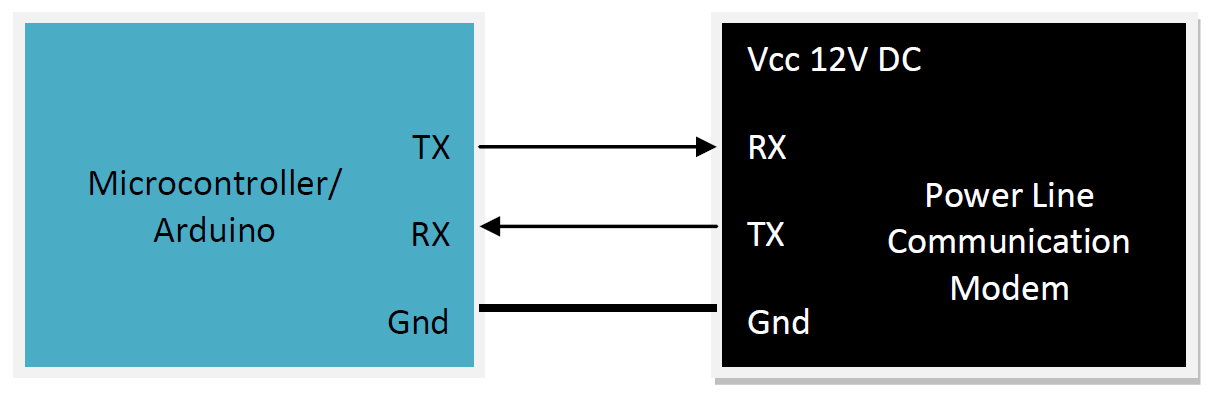
\includegraphics[scale=.8]{a}
\caption{principle1}
\label{circuit}
\end{figure}
\hspace*{1cm}This is a standard drafting table. The horizontal bar is a straight-edge which can be moved up and down by the user. The criss-cross pattern of the cables stabilizes the bar and keeps it horizontal.
\begin{figure}[h!]
\centering
\includegraphics[scale=.8]{bc}
\caption{principle2}
\label{circuit}
\end{figure}
\newpage
\hspace*{1cm}
This effect can be seen by following the direction of motion of the two cables which comprise the mechanism. Note that all of the vertical arrows point in the same direction.\\\
\begin{figure}[h!]
\centering
\includegraphics[scale=.8]{cd}
\caption{principle3}
\label{circuit}
\end{figure}
\hspace*{1cm}You could imagine attaching a stepper motor to one of the pulleys. Now, the horizontal bar can be moved up and down under computer control. This might be called a single-axis CNC stage.\\\
\begin{figure}[h!]
\centering
\includegraphics[scale=.8]{ef}
\caption{principle4}
\label{circuit}
\end{figure}
\hspace*{1cm}How might we modify this mechanism to convert it into a two-axis CNC stage? The illustrated mechanism above is one solution. Rotating both motors in the same direction results in horizontal motion. Rotating both motors in opposite directions results in vertical motion.\\\
\section{Reference Mechanism}
\hspace*{1cm}This reference mechanism is functionally identical to the last figure in the prior section. Two additional pulleys have been added to shift the belt cross-over outside of the working envelop
\begin{figure}[h!]
\centering
\includegraphics[scale=.8]{reference}
\caption{reference}
\label{circuit}
\end{figure}
\newpage
\chapter{{TOOLS AND TOOL MOUNT}}
\section{Universal Tool Mount}
\hspace*{1cm} The Universal Tool Mount (UTM) allows FarmBot  to automatically switch tools in order to perform different operations. It is a plastic component that mounts to the z-axis aluminum extrusion using two M5 screws and tee nuts. Switching of the tools is done with the help of a servo motor in the prototype.When going on a advanced scale with large number of tools an electromagnet can be used to automatically select the tools.Fig.6.1
\section{Seed Injector and Vacuum Pump}
\hspace*{1cm} The seed injector works by using a vacuum pump to suction-hold a single seed at the end of a needle. Fig.6.2 Fig.6.3\\\
\section{Moisture Sensor}
\section{Watering Nozzle and Solenoid Valve}
\hspace*{1cm}The watering nozzle accepts a concentrated stream of water coming from the UTM and turns it into a gentle shower for your plants .Fig.6.5\\\
\chapter{WORKING OF FARMBOT}
\hspace*{1cm}The block diagram of the Farmbot system is as shown in the Figure 7.1. 
\begin{figure}[h!]
\centering
\includegraphics[scale=.8]{wor}
\caption{Block diagram of Farmbot and its Android phone remote}
\label{circuit}
\end{figure}
\hspace*{1cm}
The flow charts for the software part of the Embedded System as well as the Android application are shown below.
\begin{figure}[h!]
\centering
\includegraphics[scale=.8]{qwer}
\caption{robert control application figure}
\label{circuit}
\end{figure}
\begin{figure}[h!]
\centering
\includegraphics[scale=.8]{asdf}
\caption{Embedded System program}
\label{circuit}
\end{figure}
\chapter{{RESULTS AND CONCLUSION}}
\hspace*{1cm} Implementation of the wireless control is done with the help of the Bluetooth HC-05 module. Controlling of the various modules (motors) are done by receiving the commands over the Bluetooth from Android mobile application. Once the commands are received, the microcontroller sends a digital signal to the respective port pins in the microcontroller, these are in turn connected to the enable pins of  the Motor driver boards, which drive the respective motors. The figure 6.1 shows the FarmBot with all the different components labelled. The robot designed in this project is connected to the user mobile phone over Bluetooth link therefore it is limited to the Bluetooth range, this can be extended with the help of a GSM module in the place of a Bluetooth receiver.When the application is first launched, the user is greeted with a login screen that can be unlocked by entering the username and password. The application also displays required notifications to display the current command being transmitted to the Microcontroller via Bluetooth. The agriculture automation system has been designed and realized using a simple model controlled over the Bluetooth signal from Android Mobile Phone. The designed system is a low cost demonstration model, which is able to convey the application and future scope for modular automated agriculture systems. This demonstration system was made at a low cost and was tested successfully to grow small crops.
\chapter {SOCIAL RELEVANCE}
\hspace*{1cm}Commercially, farms -big and small can use FarmBot to reduce labor, improve efficiency, control inputs and test new growing method. \\\

\hspace*{1cm}*FarmBot produces 25 percentage fewer carbon dioxide than standard national food production.\\\
\hspace*{1cm}	*FarmBot helps in effective weed control. \\\
\hspace*{1cm}	*Farm bot can be setup on any terrain like on a raised bed, rooftop or in a greenhouse to grow food for yourself, your family and your community.\\\
\hspace*{1cm}	*It helps in the growth of dying agriculture in urban areas. Development in agriculture is important for the improvement of the financial state of the nation. \\\
\hspace*{1cm}  *FarmBot grown veggies are significantly less expensive than veggies purchased at the grocery stores. \\\
\hspace*{1cm}	*FarmBot reduce the risk of working in unsafe conditions like splashing chemicals and pesticides. \\\
\hspace*{1cm}
This project is a response to the increase in food production needed due to the growth in world population and the potential of precision agriculture to reduce the environmental impact of farming by reducing water use, energy, transportation, petrochemicals and time required to grow crop.\\\
\chapter{FUTURE WORK}
\hspace*{1cm}•	Weeding mechanism can be incorporated in which a camera can be mounted on the z axis and can be used to detect any plants in positions other than where seeds are sown and consider them as weeds. Then a weeding tool can be used to suppress the weed under the soid by pushing them under the soil.
•	Farmbot can be made Solar Powered which can reduce the use of electricity.
•	Rainwater harvesting tank can be made along with the Farmbot to collect water during rainy season and meet the farm requirement in summer.
•	Night lighting can be provided for security.\\\
\chapter{PROGRAM CODE}

\begin{thebibliography}{99}
\addcontentsline{toc}{chapter}{{ References}}

\bibitem{}  Narendra Limbu, Indrajit Ahuja, Harshal Sonar, Sudeep Solanki, Soniya Jain, Hoam Chung, Debraj Chakraborty, "Outdoor Co-operative Control Of Multiple Quadcopters using decentralized
GPS localisation", \textbf{\emph{IEEE 10th International Workshop on Robot Motion and Control, July 6-8, 2015 }}

\bibitem{} Dror Epstein and Dan Feldman, "Quadcopter Tracks Quadcopter via Real-Time Shape Fitting",\textbf{\emph{IEEE Robotics and Automation Letters, VOL. 3, NO. 1, January 2018} }

\bibitem{}  Sonia Waharte and Niki Trigoni[3],"Supporting Search and Rescue Operations with
UAVs",\textbf{\emph{2010 International Conference on Emerging Security Technologies, 7 Sept. 2010}}

\bibitem{} Anjan Chakrabarty and Robert Morris, "Autonomous Indoor Object Tracking with the Parrot AR.Drone", \textbf{\emph{International Conference on Unmanned Aircraft Systems (ICUAS) June 7-10, 2016}}

\bibitem{} Yu-chia Chung and Zhihai, "Low complexity and reliable moving objects detection and tracking for aerial video surveillance using small UAVs" , \textbf{\emph{Proceedings of
the IEEE , Volume: 89 Issue: 10 Oct 2007}}

\bibitem{}  Artem Rozantsev and Vincent Lepetit, "Detection of flying objects such as Unmanned Aerial Vehicles (UAVs) and aircrafts", \textbf{\emph{Pattern Analysis and Machine Intelligence,
IEEE Transactions on Volume: 23 Issue: 8 Aug 2001
,pp.873-889 }}

\bibitem{} J. Redmon, S. Divvala, R. Girshick, and A. Farhadi, “Unified, real-time object detection”, \textbf{\emph{ Proceedings of the IEEE Conference on Computer Vision and Pattern Recognition, 2016, pp. 779-788.}}


\end{thebibliography}




\end{document}

